\documentclass{standalone}
\usepackage{tikz}
\usepackage{pgfplots}
\pgfplotsset{width=32cm,height=18cm,compat=1.3}
\pgfplotsset{every tick label/.append style={font=\Huge}}
\usepackage{filecontents}

\usetikzlibrary{patterns}

\definecolor{citrine}{rgb}{0.89, 0.82, 0.04}

\begin{document}
	\centering
		\vspace{1.5em}
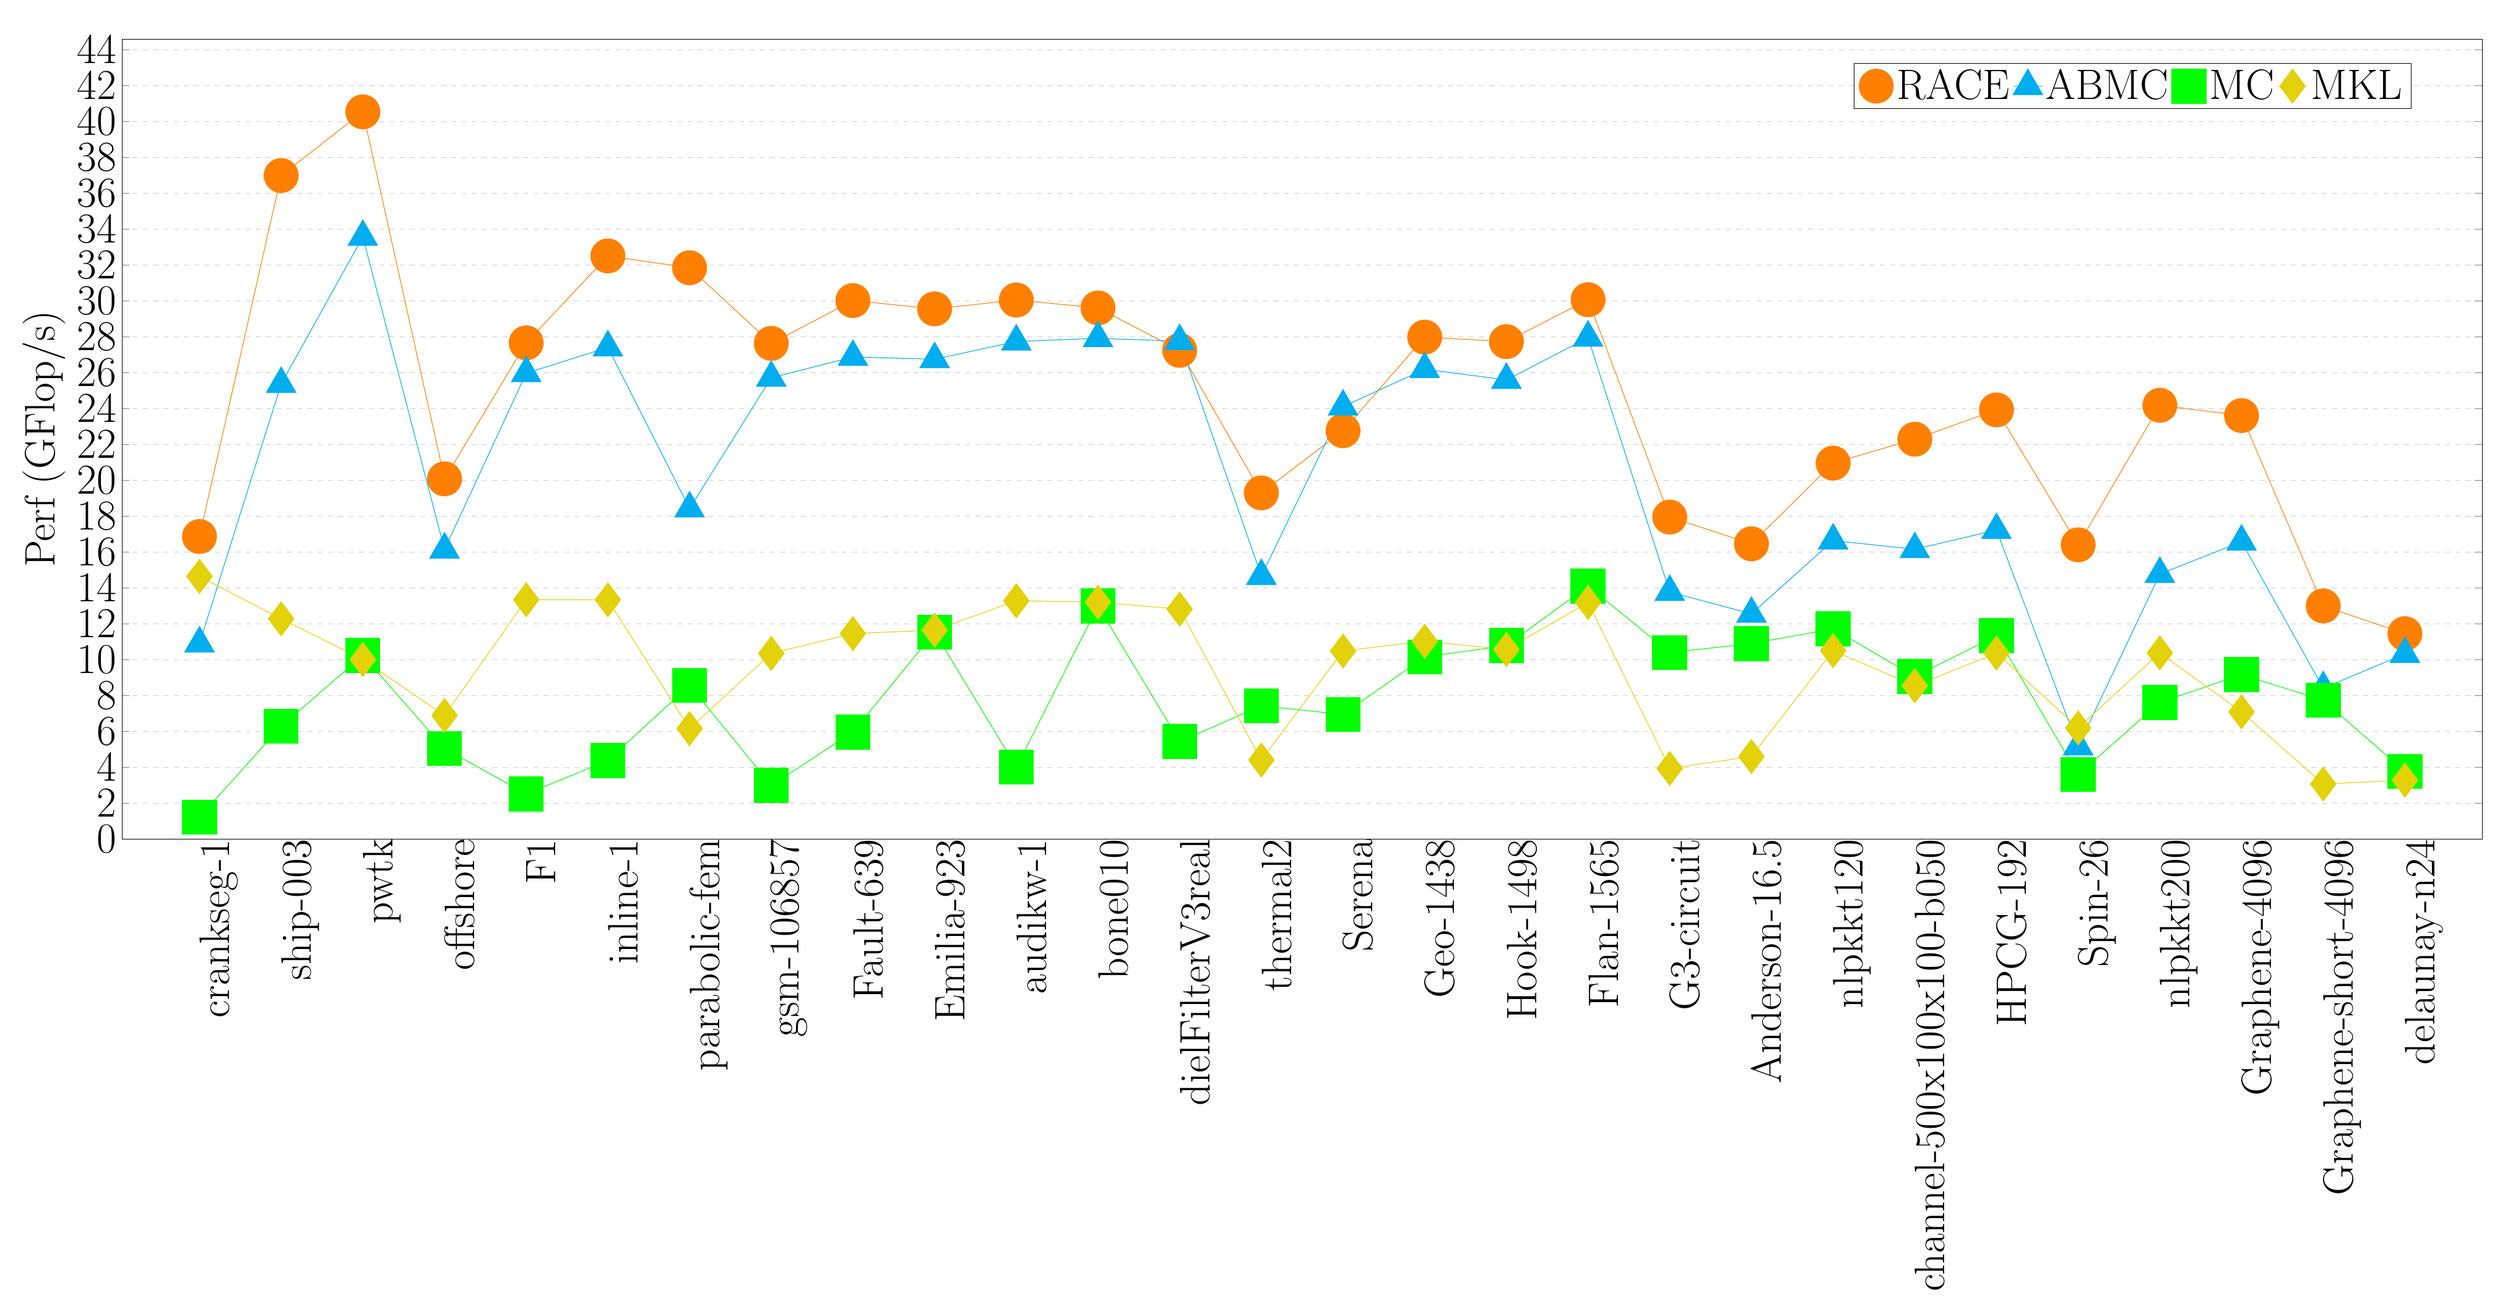
\begin{tikzpicture}
		%	\node at (13.25,15) {\LARGE{}};
			\begin{axis}[
		%	xmin=0.25, xmax=7.25,
			ymin=0, %ymax=3.25,
			xtick={1, 2, 3, 4, 5, 6, 7, 8, 9, 10, 11, 12, 13, 14, 15, 16, 17, 18, 19, 20, 21, 22, 23, 24, 25, 26, 27, 28},
		%	ytick={0,0.5,1,1.5,2,2.5,3},
			xticklabels={crankseg-1, ship-003, pwtk, offshore, F1, inline-1, parabolic-fem, gsm-106857, Fault-639, Emilia-923, audikw-1, bone010, dielFilterV3real, thermal2, Serena, Geo-1438, Hook-1498, Flan-1565, G3-circuit, Anderson-16.5, nlpkkt120, channel-500x100x100-b050, HPCG-192, Spin-26, nlpkkt200, Graphene-4096, Graphene-short-4096, delaunay-n24},
			width  = 50cm,
			height = 18cm,
			major x tick style = transparent,
			%	minor ytick={1, 5, 10, 15, 20, 25, 30 ,35,40},
			grid = minor,	
			%add_bar_commands
			ymajorgrids = true,
			grid style={dashed, gray!40},
			ylabel = {\Huge{Perf (GFlop/s)}},
		%	symbolic x coords={Graphene-2048-2048, Graphene-4096-4096, Spin-24-24-24},
			x tick label style={rotate=90, anchor=north east, inner sep=0mm, font={\Huge}},
			tick label style={font={\Huge}},
			scaled y ticks = false,
			enlarge x limits=0.035,
			legend cell align=left,
			legend style={font=\Huge},
			legend columns=-1,
			legend style={
				%at={(1,1.05)},
				%anchor=south east,
				%column sep=1ex,
				legend pos=north east
			},
			%spl_legend_code
			title= {\Huge\scalebox{1.5}{{}}}
			]

\addplot[mark=*, mark size=10pt, mark options={orange}, draw=orange ] plot coordinates{(1,16.854992) (2,36.979831) (3,40.528888) (4,20.072225) (5,27.650065) (6,32.497825) (7,31.837543) (8,27.622948) (9,30.008732) (10,29.544466) (11,30.038410) (12,29.598056) (13,27.233392) (14,19.287252) (15,22.750551) (16,27.971316) (17,27.719366) (18,30.058614) (19,17.938689) (20,16.449635) (21,20.948219) (22,22.279768) (23,23.914583) (24,16.392259) (25,24.170988) (26,23.598034) (27,12.986649) (28,11.440436)};
\addplot[mark=triangle*, mark size=10pt, mark options={cyan}, draw=cyan ] plot coordinates{(1,10.89111) (2,25.357945) (3,33.554455) (4,16.126065) (5,25.959287) (6,27.395207) (7,18.41691) (8,25.702073) (9,26.866035) (10,26.738884) (11,27.723627) (12,27.906569) (13,27.743464) (14,14.652735) (15,24.094638) (16,26.184645) (17,25.584772) (18,27.937259) (19,13.762619) (20,12.544985) (21,16.628392) (22,16.146198) (23,17.215598) (24,5.153603) (25,14.764235) (26,16.566482) (27,8.40312) (28,10.30723)};
\addplot[mark=square*, mark size=10pt, mark options={green}, draw=green ] plot coordinates{(1,1.217100) (2,6.273317) (3,10.223248) (4,5.038080) (5,2.503908) (6,4.370578) (7,8.560793) (8,2.979327) (9,5.953189) (10,11.526041) (11,4.003217) (12,12.984448) (13,5.433710) (14,7.412819) (15,6.938383) (16,10.146493) (17,10.772068) (18,14.094140) (19,10.385653) (20,10.887933) (21,11.705998) (22,9.056057) (23,11.328209) (24,3.584046) (25,7.610445) (26,9.154874) (27,7.734495) (28,3.762009)};
\addplot[mark=diamond*, mark size=10pt, mark options={citrine}, draw=citrine ] plot coordinates{(1,14.632991) (2,12.267928) (3,9.998300) (4,6.880652) (5,13.331976) (6,13.325569) (7,6.145878) (8,10.339662) (9,11.446922) (10,11.637173) (11,13.275046) (12,13.198980) (13,12.808297) (14,4.394268) (15,10.476069) (16,11.017262) (17,10.559251) (18,13.180780) (19,3.927535) (20,4.589667) (21,10.494941) (22,8.535902) (23,10.356665) (24,6.187077) (25,10.368500) (26,7.079533) (27,3.059906) (28,3.271750)};
	%addplot cmd

	\legend{RACE, ABMC, MC, MKL}

	\end{axis}			
\end{tikzpicture}

\end{document}

